\documentclass[avery5371, grid,frame]{flashcards}

\usepackage{graphicx}
\usepackage{geometry}

\geometry{a4paper, landscape}
\cardfrontstyle[\large\slshape]{headings}
\cardbackstyle{empty}

\begin{document}

\renewcommand{\cardpaper}{a4paper}
\renewcommand{\cardpapermode}{landscape}
\renewcommand{\cardrows}{2}
\renewcommand{\cardcolumns}{2}
\setlength{\cardheight}{3.5in}
\setlength{\cardwidth}{5.0in}
\setlength{\topoffset}{0.65in}
\setlength{\oddoffset}{0.65in}
\setlength{\evenoffset}{0.65in}

\begin{flashcard}{area}
    \vspace*{\fill}
    \begin{center}
        \begin{minipage}[c]{.45\textwidth}
            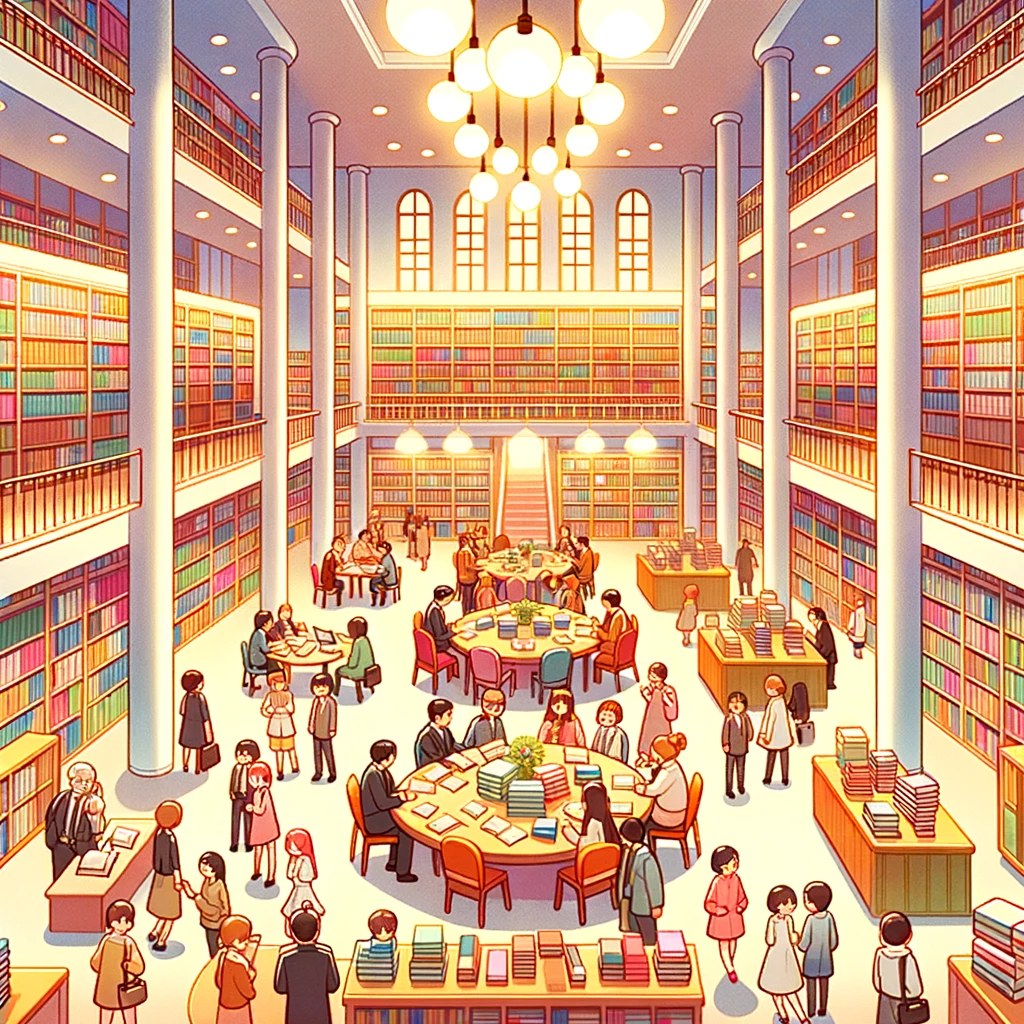
\includegraphics[width=\textwidth]{cards/a/area/area - A big library with various sections, and people are gathered for reading.png}
        \end{minipage}
        \begin{minipage}[c]{.45\textwidth}
            \begin{itemize}\setlength\itemsep{12pt}
            \item Explanation: \ A part or section within a larger place

            \item Example: \ A big library with various sections, and people are gathered for reading
            \end{itemize}
        \end{minipage}
    \end{center}
    \vspace*{\fill}
\end{flashcard}\begin{flashcard}{area}
    \vspace*{\fill}
    \begin{center}
        \begin{minipage}[c]{.45\textwidth}
            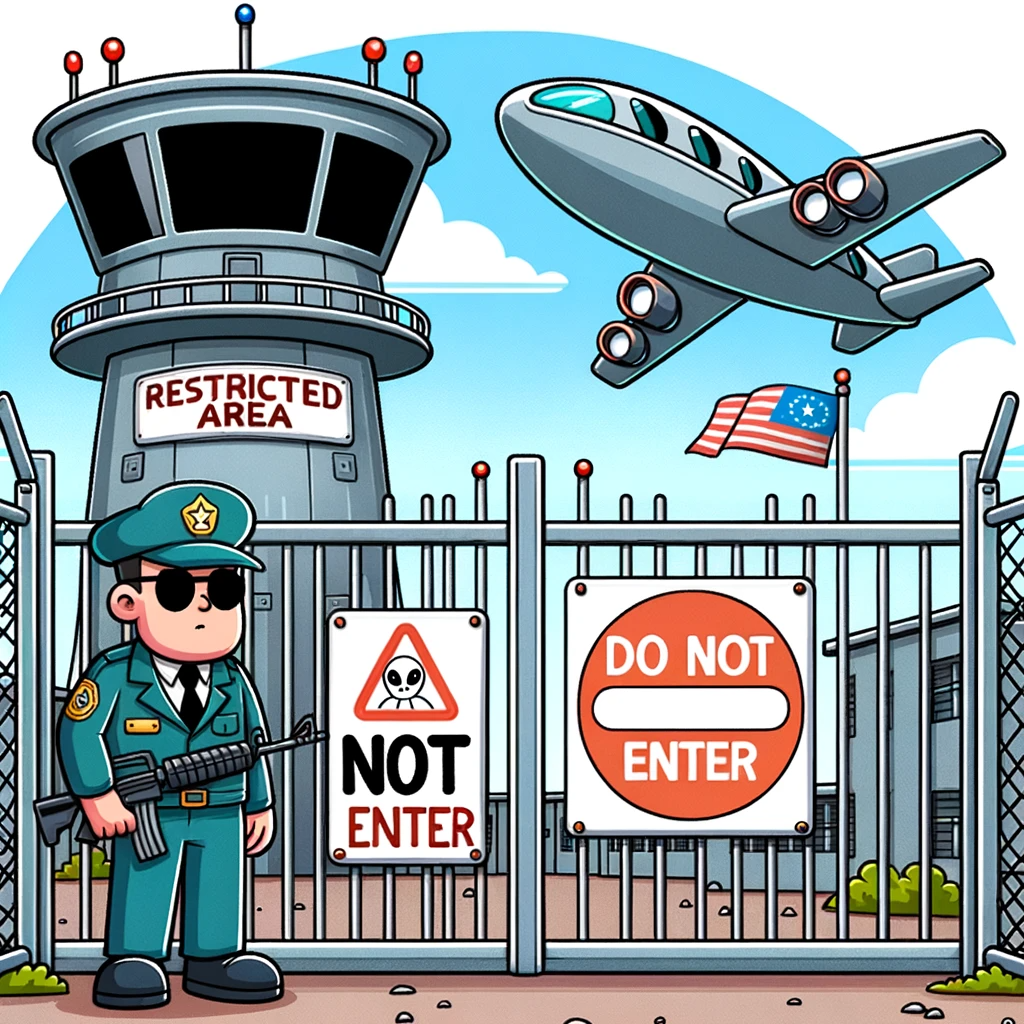
\includegraphics[width=\textwidth]{cards/a/area/area - a restricted zone with a 'Do Not Enter' sign and a guarded gate.png}
        \end{minipage}
        \begin{minipage}[c]{.45\textwidth}
            \begin{itemize}\setlength\itemsep{12pt}
            \item Explanation: \ A part or section within a larger place

            \item Example: \ a restricted zone with a 'Do Not Enter' sign and a guarded gate
            \end{itemize}
        \end{minipage}
    \end{center}
    \vspace*{\fill}
\end{flashcard}\begin{flashcard}{area}
    \vspace*{\fill}
    \begin{center}
        \begin{minipage}[c]{.45\textwidth}
            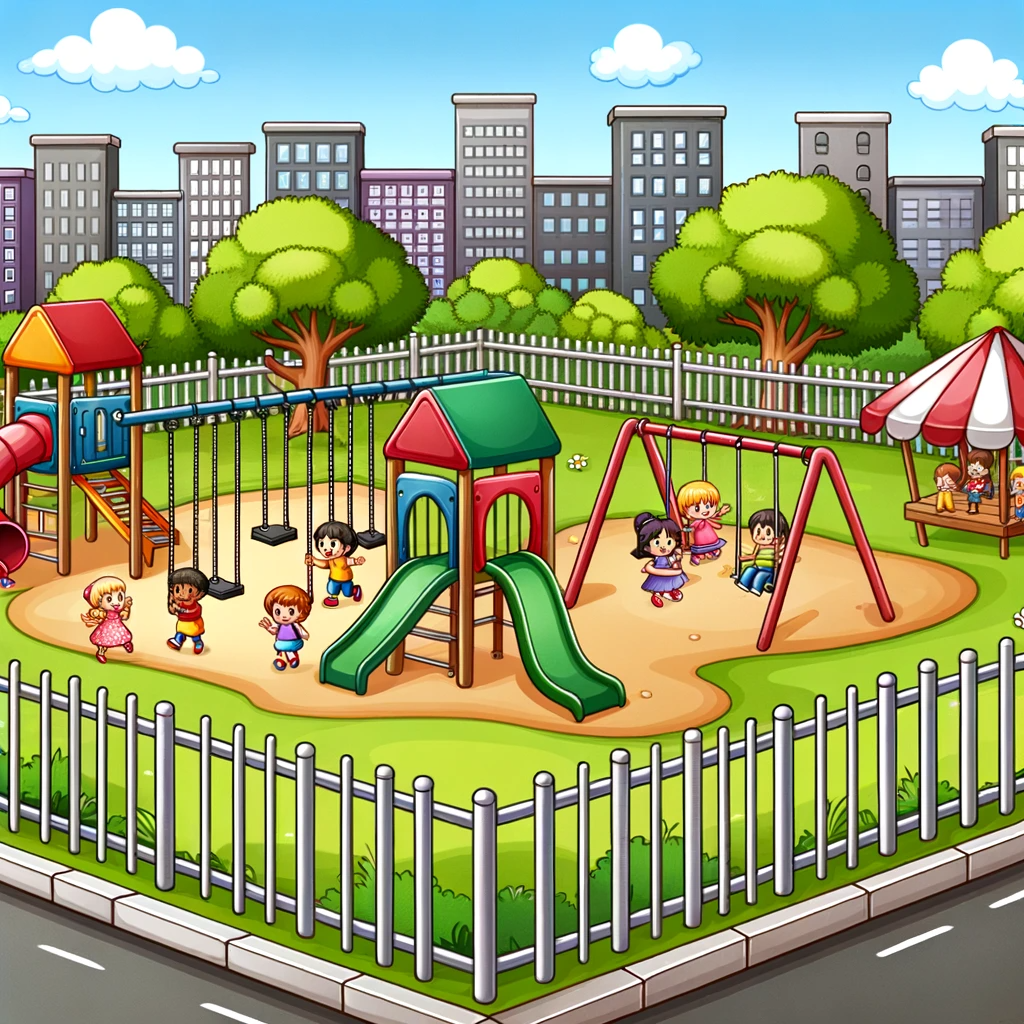
\includegraphics[width=\textwidth]{cards/a/area/area - a fenced playground with swings, slides, and kids playing.png}
        \end{minipage}
        \begin{minipage}[c]{.45\textwidth}
            \begin{itemize}\setlength\itemsep{12pt}
            \item Explanation: \ A part or section within a larger place

            \item Example: \ a fenced playground with swings, slides, and kids playing
            \end{itemize}
        \end{minipage}
    \end{center}
    \vspace*{\fill}
\end{flashcard}\begin{flashcard}{area}
    \vspace*{\fill}
    \begin{center}
        \begin{minipage}[c]{.45\textwidth}
            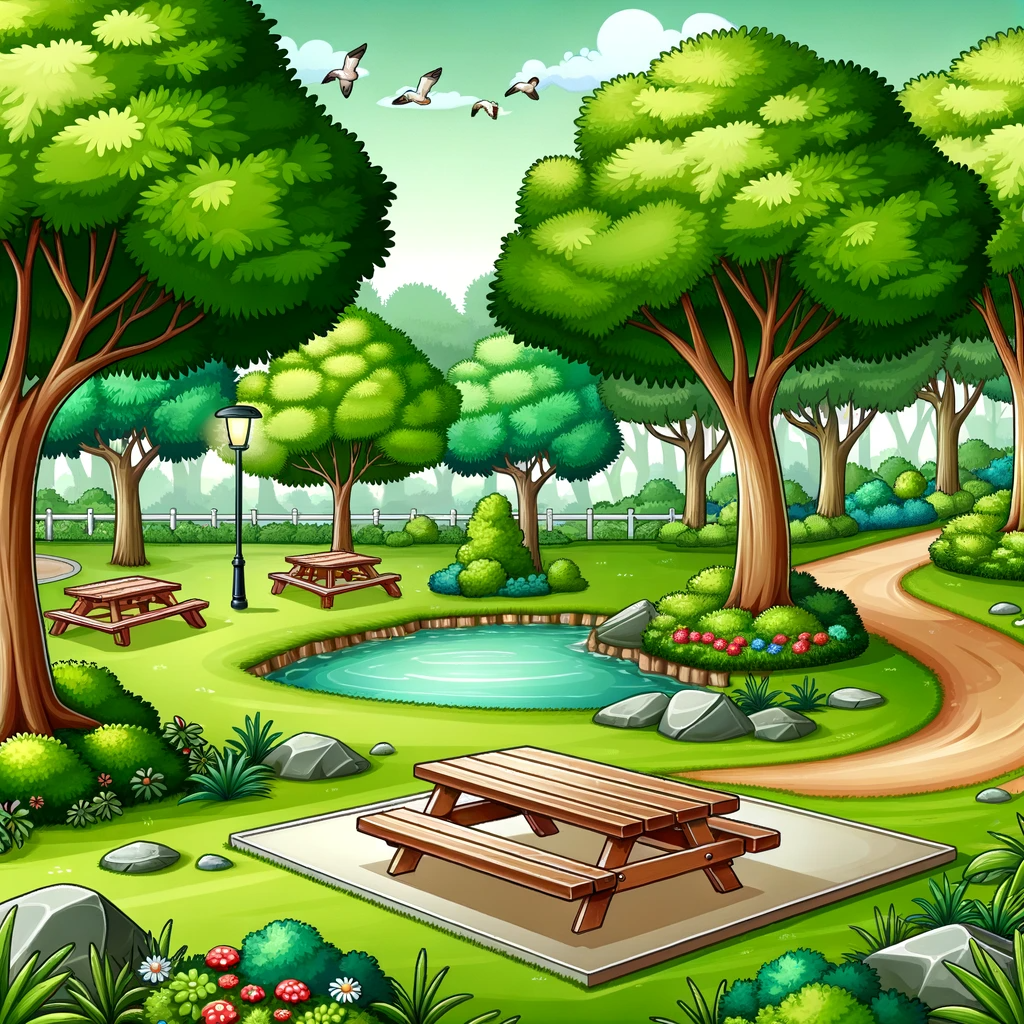
\includegraphics[width=\textwidth]{cards/a/area/area - a serene picnic area in a park with trees, benches, and a pond.png}
        \end{minipage}
        \begin{minipage}[c]{.45\textwidth}
            \begin{itemize}\setlength\itemsep{12pt}
            \item Explanation: \ A part or section within a larger place

            \item Example: \ a serene picnic area in a park with trees, benches, and a pond
            \end{itemize}
        \end{minipage}
    \end{center}
    \vspace*{\fill}
\end{flashcard}

\end{document}